\documentclass{article}

\usepackage{graphicx}
\usepackage{extarrows}

\usepackage{listings}
\usepackage[framed,numbered,autolinebreaks,useliterate]{mcode}
\lstset{language=Matlab}

\usepackage{multirow}
\usepackage{makecell}
\usepackage{booktabs}
\usepackage{cite}
\usepackage{geometry}
\usepackage{pythonhighlight}
\usepackage {subcaption}
\usepackage{setspace}
\usepackage{indentfirst}
\usepackage{ragged2e}
\usepackage{amsmath}
\usepackage{bm}
\geometry{a4paper, scale=0.75}
\newcommand{\upcite}[1]{\textsuperscript{\textsuperscript{\cite{#1}}}}

\title{Support Vector Machine with Line Search SQP using a flexible step acceptance strategy}
\author {Meijia Liu}

\begin{document}
\maketitle


\begin{spacing}{1.5}


\newpage
\setcounter{page}{1}
\tableofcontents
\newpage
\section{Introduction}
The Support Vector Machine(SVM) is one of the machine learning techniques that can help to solve classification problems. It s a linear classifier that can be viewed as an extension of the perceptron, which guaranteed to find a hyperplane if it exists. However, if there is no separating hyperplane between two classes because of low dimension, the linear boundary is not feasible. As a result, we allow some misclassifications and use soft margin for classifier. This report will solve linear non-separable case and use Line Search Subsequence Quadratic Programming algorithm to find optimal hyperplane.

\section{Support Vector Machine}
\subsection{Linear Separable SVM}
The classification problem can be represented as follows. Let $S=\{(\bm{x}_i,y_i)\}^m_{i=1}\in \bm{R}^n$ be a training set,  in binary classification the set of label is $\{-1,1\}$. A hyperplane means a set $H_{\bm{w},b}=\{\bm{x}\in \bm{R}^n: \bm{w}^T\bm{x}+b=0\}$, where $\bm{w}\in\bm{R}^n$ and $b\in\bm{R}$.  The value of each $w_i$ is a measure of the importance of each attribute for the classification problem and $b$ is a bias value.\par

The objective is to maximize the distance between hyperplane and the closest point within both classes, which also named 'margin', under the constraints that all data points lie on the correct side of the hyperplane. It solves optimization problem:
\begin{align}
H(S):=\max_{\bm{w},b} \min_{1\le i \le m}\{\frac{y_i(\bm{w}^T\bm{x}_i+b)}{||\bm{w}||}: y_j(\bm{w}^T\bm{x}_j+b\ge 0), j=1,\cdots,m\}>0
\end{align}
where $\frac{y_i(\bm{w}^T\bm{x}_i+b)}{||\bm{w}||}$ is the distance of a point $x$ from the hyperplane $H_{\bm{w},b}$. In this report we choose to work with Canonical hyperplane. Canonical hyperplane require that $min^m_{i=1}y_i(\bm{w}^T\bm{x}_i)=1$\upcite{Ref5}, we have:
\begin{align}
H(S)&=\max_{w,b}\{\frac{1}{||\bm{w}||}: \min_{i}\{y_i(\bm{w}^T\bm{x}_i+b)\}=1, y_i(\bm{w}^T\bm{x}_i+b)\ge0 \}\\
&=\max_{w,b}\{\frac{1}{||\bm{w}||}: y_i(\bm{w}^T\bm{x}_i+b)\ge 1\}
\end{align}
Then the optimal hyperplane can be constructed by solving the following constrained quadratic optimization primal problem:
\begin{align}
&Minimize\quad \frac{1}{2}\bm{w}^T\bm{w}\\
&subject\ to \quad y_i(\bm{w}^T\bm{x}_i+b)\ge1, i=1,\cdots,m
\end{align}

\subsection{Linear non-separable SVM}
If the data cannot be separated by a hyperplane perfectly, we can fix this by allowing some misclassification with the introduction of slack variables\upcite{Ref3}:
\begin{align}
&Minimize\quad \frac{1}{2}\bm{w}^T\bm{w}+C\sum^n_{i=1}\xi_i\\
&subject\ to \quad y_i(\bm{w}^T\bm{x}_i+b)\ge1-\xi,\quad \xi_i\ge0
\end{align}
$C$ is complexity constants and $\xi_i$ denotes the misclassification loss, here we replace $\xi_i$ by the hinge loss:
\begin{align}
\xi_i=\left\{
\begin{aligned}
1-y_i(\bm{w}^T\bm{x}_i+b)&\quad y_i(\bm{w}^T\bm{x}_i+b)<1\\
0 &\quad y_i(\bm{w}^T\bm{x}_i+b)\ge1
\end{aligned}
\right.
\end{align}

Substitute (8) into equation (6), we obtain the following unconstrained version as loss function and regularizer:
\begin{align}
\min_{w,b}\quad \bm{w}^T\bm{w}+C\sum^n_{i=1}max[1-y_i(\bm{w}^T\bm{x}+b),0]
\end{align}

\subsubsection{New dual form}
The solution of equation (6) combined with inequation (7) is equivalent to find the saddle point of the Lagrangian function
\begin{align}
L(\bm{w},\bm{\xi},b; \bm{\alpha},\bm{\beta})=\frac{1}{2}\bm{w}^T\bm{w}+C\sum^m_{i=1}\xi_i-\sum^m_{i=1}\alpha_i[y+i(\bm{w}^T\bm{x}_i+b)+\xi_i-1]-\sum^m_{i=1}\beta_i\xi_i
\end{align}
where $\alpha_i,\ \beta_i\ge0$ are the Lagrange multipliers.
We minimize $L$ over $\bm{w},\ \bm{b}\ and\ \bm{\xi}$ and obtain:
\begin{align}
\frac{\partial L}{\partial b}&=\sum^m_{i=1}y_i\alpha_i=0\\
\frac{\partial L}{\partial \bm{w}}&=\bm{w}-\sum^m_{i=1}\alpha_i y_i\bm{x}_i=\bm{0}\\
\frac{\partial L}{\partial\xi_i}&=C-\alpha_i-\beta_i=0
\end{align}
Then dual problem shows\upcite{Ref2}:
\begin{align}
\min_{\alpha_1,\cdots,\alpha_n}&\quad \frac{1}{2}\sum_{i,j}\alpha_i\alpha_jy_iy_j<x_i,x_j>-\sum_{i=1}\alpha_i\\
s.t.&\quad 0\le\alpha_i\le C\\
&\quad \sum^n_{i=1}\alpha_iy_i=0
\end{align}

\subsubsection{Kernel Tricks}
For a non-linear classification problem in the input space, it can be transformed into a linear classification problem in some dimensional feature space by means of a non-linear transformation to train a linear support vector machine in a high-dimensional feature space. Since both the objective function and the classification decision function involve only the inner product between instances in a pairwise problem learned by a linear support vector machine, it is not necessary to explicitly specify the non-linear transformation, but to replace the inner product with a kernel function. \par

According to Somla et al.(1998)\upcite{Ref6}, under general smoothness assumption, gaussian kernel tend to perform well and should be considered if no additional information could obtained from data. Gaussian kernel, also known as RBF kernel: 
\begin{align}
K(x,z)=exp(\frac{-||x-z||^2}{2\sigma^2})
\end{align}
As a result, our new dual problem under kernel trick is:
\begin{align}
\min_{\alpha_1,\cdots,\alpha_n}&\quad \frac{1}{2}\sum_{i,j}\alpha_i\alpha_jy_iy_jK_{ij}-\sum_{i=1}\alpha_i\\
s.t.&\quad 0\le\alpha_i\le C\\
&\quad \sum^n_{i=1}\alpha_iy_i=0
\end{align}
where $\bm{w}=\sum^n_{i=1}\alpha_iy_i\phi(x_i)$ and prediction:
\begin{align}
h(x)=sign(\sum^n_{i=1}\alpha_iy_ik(\bm{x}_i,x)+b)
\end{align}

\subsection{Support Vectors}
Support vectors are those points satisfies:
\begin{align}
y_i(\bm{w}^T\phi(xi)+b)=1
\end{align}
and the complementary KKT-conditions says $\alpha(y_i(\bm{w}^T\phi(xi)+b)-1)=0$ and $\alpha\ge0$. Equation (22) shows that $y_i(\bm{w}^T\phi(xi)+b)-1\neq0$ for training inputs without support vectors, then to satisfy KKT conditions, $\alpha_i=0$ has to be satisfied. As a result, $\alpha_i>0$ for support vectors. This lead to a nice interpretation of the dual problem, where $h(x)$ is equivalent to the sum of all support vectors and all inputs $\bm{x}_i$ with nonzero alpha can be discarded after training.

\subsection{Recovering b}
The bias term is indeed, a special term in SVM which controls whether hyperplane pass through the original point. The bias term should be treated separately because bias term is no longer part of our dual optimization problem. As we mentioned before, in the dual, support vectors are those with $\alpha_i>0$. we can calculate $b$ from support vectors:
\begin{align}
b=y_i-\sum_jy_j\alpha_jk(\bm{x}_j, \bm{x}_i)
\end{align}

\section{Line Search SQP}
Recall last section, we need to optimize:
\begin{align}
\min_{\alpha_1,\cdots,\alpha_n}&\quad \frac{1}{2}\sum_{i,j}\alpha_i\alpha_jy_iy_jK_{ij}-\sum_{i=1}\alpha_i\\
s.t. &\quad \sum^n_{i=1}\alpha_iy_i=0\\
&\quad \forall i\ \alpha_i\ge0\\
&\quad \forall i\ C-\alpha_i\ge0
\end{align}
It is a constraint optimization problem with both equality and inequality linear constrains. The objective function is a quadratic programming and the problem is deterministic. The challenging for this problem is it has inequality constrains and more than one. \par

In this report we will use Line Search SQP method given by Wright and Nocedal(1999)\upcite{Ref7} and modified it with a flexible step acceptance strategy raised by Zhu and Pu(2012)\upcite{Ref8}.

\subsection{Equality Constraints}
This subsection start from equality-constrained problem:
\begin{align}
&min\quad f(\bm{x})\\
&s.t\quad c(\bm{x})=\bm{0}
\end{align}

Define $A(\bm{x})=\bigtriangledown c(\bm{x})=[\bigtriangledown c_1, \cdots, \bigtriangledown c_m]\in R^{n\times m}$, is a Jacobian matrix of $c(\bm{x})$\par
~\par
\textbf{SQP framework:}\par
At step $x_k$, assume $f(x_k)$ is not optimal, hence we expect that the value $f(x_k+p)$ should decrease with respect to the descent direction in k-th step $p$. Additionally, $x_k+p$ should still in feasible set $D$, then we get a new subproblem which minimize $f(x_k+p)$:
\begin{align}
\min_p&\quad f(x_k+p)\\
s.t. &\quad c(x_k+p)=0
\end{align}
Through second-order and first-order Taylor expansion for (30) and (31), our subproblem is almost equivalent to:
\begin{align}
\min_p&\quad f_k+\bigtriangledown f_k^Tp+\frac{1}{2}p^T\bigtriangledown^2f(x)p\\
s.t. &\quad c_k+\bigtriangledown c_k^Tp=0
\end{align}

The Lagrangian for this problem is:
\begin{align}
L(p,\lambda)=f_k+\bigtriangledown f_k^Tp+\frac{1}{2}p^T\bigtriangledown^2f(x)p-\lambda^T(c_k+\bigtriangledown c_k^Tp)
\end{align}
where $\mu\in R^m$ is the Lagrangian multiplier for equality constraint. The KKT conditions for this problem are:
\begin{align}
\left\{
\begin{aligned}
&\bigtriangledown_pL(p,\lambda)=0\\
&\ c_k+\bigtriangledown c_k^Tp=0
\end{aligned}
\right.
\end{align}
which is equivalent to:
\begin{align}
F(p,\lambda)=
\begin{bmatrix}
\bigtriangledown_pL(p,\lambda)\\
\ c_k+\bigtriangledown c_k^Tp
\end{bmatrix}
=\bm{0}
\end{align}
We then apply Newton-Raphson Iteration Method $\bigtriangledown^TF(x_k)p=-F(x_k)$ to calculate the zero points of (36). Then we have:
\begin{align}
\begin{bmatrix}
\bigtriangledown_{pp}L(p,\lambda)-\bigtriangledown c_k\\
\bigtriangledown c_k
\end{bmatrix}
\begin{bmatrix}
p_{xk}\\
p_{\lambda k}
\end{bmatrix}
=
\begin{bmatrix}
-\bigtriangledown_pL(p,\lambda)\\
c_k+\bigtriangledown c_k^Tp
\end{bmatrix}
\end{align}
at one particular iteration step $p_k$

\noindent This is a sufficient and necessary condition for the following quadratic optimal problem:
\begin{align}
&\min_p\quad g_k^Tp+\frac{1}{2}p^TH_kp\\
&s.t.\quad A_k^Tp+c_k=0
\end{align}
where $A_k=\bigtriangledown c_k$, $g_k$ is gradient Lagrangian and $H_k$ is a symmetric approximation to the current Lagrangian Hessian.
Apply the subsequence quadratic optimal problem consist of objective function (36) and constraints (37) in each iteration to the new iterate $(x_{k+1},\ \lambda_{k+1})$ is the basic and simplest form of SQP method.\par

\subsection{Inequality Constraints}
According to our final SVM soft margin dual optimization problem (24)-(27), we can write the constraint problem in the following general form:
\begin{align}
\min_{\alpha}&\quad f(\alpha)\\
s.t. &\quad c_\epsilon(\alpha)=0\\
&\quad c_I(\alpha)\ge0
\end{align}
where $\alpha\in R^n$, $\epsilon=\{i|i=1,2,\cdots,m_e\}$ and $I=\{i|i=m_e+1,\cdots,m\}$, $f: R^n\to R$ and $c: R^n\to R^m$ are smooth functions. The Lagrangian for this constraint problem is:
\begin{align}
L(x,\lambda,\mu)=f(\alpha)-\lambda^Tc_\epsilon(\alpha)-\mu^Tc_I(\alpha)
\end{align}
and its KKT conditions are:
\begin{align}
\left\{
\begin{aligned}
&\bigtriangledown f(\alpha)-A_\epsilon^T\lambda-A_I^T\mu=0\\
&\ c_\epsilon(\alpha)=0\\
&\ c_I(\alpha)\ge0\\
&\ \mu\ge0\\
&\ \mu^Tc_I(x)=0
\end{aligned}
\right.
\end{align}
Extended from (38) and (39) in equality constraints, the new iterate $(x_{k+1}, \lambda_{k+1})$ can therefore be defined as he solution of the quadratic program:
\begin{align}
\min_p &\quad g_k^Tp+\frac{1}{2}p^TH_kp\\
s.t.&\quad A_{\epsilon k}^Tp+c_{\epsilon k}=0\\
&\quad A_{Ik}^Tp+c_{Ik}\ge0
\end{align}

According to Wright and Nocedal(1999), this ensures local convergence since we can always convergent to optimal solution if the calculated $p_k$ is a descent direction. However, if $p_k$ is not a acceptable descent direction, our basic algorithm will not convergent to the optimal solution.\par

\subsection{Algorithm Development}
To avoid insufficient decrease descent $p_k$ in each sub-quadratic program, this report use Damped BFGS Updating\upcite{Ref7} to approximate and ensure positive definite Hessian and merit function step acceptance strategy with feasible penalty functions\upcite{Ref8} to generate step length $\alpha_k$
\subsubsection{Merit Function}
In most common SQP methods, the next iterate step length is obtained by a line search backtracking along the search direction, here we use a merit function to decide whether a trial step should be accepted. A widely used merit function is the $l_1$ penalty function\upcite{Ref8}:
\begin{align}
\phi(x;\pi_k):=f(x)+\pi_kh(x)
\end{align}
where $\pi_k$ is the current penalty parameter. Extended to inequality case\upcite{Ref9}, the flexible penalty function is:
\begin{align}
\phi(x;\pi_k)=f(x)+\pi_k||c_\epsilon(x)||_1+\pi_k||c_I(x)^-||_1
\end{align}
where $c_I(x)^-=min\{c_I(x),0\}$. 
Then the directional derivative of $\phi$ in the direction $p_k$ satisfies:
\begin{align}
D(\phi(x;\pi_k); p_k)=\nabla f(x)+\pi_k||\nabla c_\epsilon(x)||_1+\pi_k||max\{-\nabla c_I(x),0\}||_1
\end{align}
In order to ensure that $p_k$ is a descent direction, we choose $\pi_k$ such that:
\begin{align}
\pi_k=\left\{
\begin{aligned}
& \pi_{k-1}\qquad \pi_{k-1}\ge r_k\\
&r_k+\epsilon \qquad otherwise,
\end{aligned}
\right.
\end{align}
where $r_k=max\{||\lambda_k||_\infty, ||\mu_k||_\infty\}$, $\epsilon>0$ is a small constant.\\
According to Zhu and Pu(2012)\upcite{Ref8}, if we choose penalty parameter too low, we may produce an infeasible point while slow convergence when it is large.\\
According to Boggs and Tolle(1995)\upcite{1}, it must be possible to reduce $\phi$ by taking an appropriate step in the direction $p_k$ generated by solving the quadratic subproblem. This appropriate step length that decreases merit function can be computed by a backtracking procedure of choosing smaller step length until a suitable one is obtained.
In a line search method, a step $\alpha_kp_k$ will be accepted if:
\begin{align}
\phi(x_k+\tau^jp_k; \pi_k)\le\phi(x_k; \pi_k)+\eta\tau^jD(\phi(x;\pi_k);p_k)
\end{align}
where j is the j-th iteration when doing line search. After finding an optimal next iterate step length, we set $\alpha_k=\tau^{j_k}$ and update $x_{k+1}=x_k+\alpha_kp_k$.

\subsubsection{Damped BFGS Updating}
The Hessian of the Lagrangian is made up of the second derivatives of the objective function and constraints, in some situation it is hard to get enough information to compute. Besides, normal BFGS method could not ensure a positive definite approximated hessian at each step\upcite{Ref7}. That is, in BFGS method, we update $H_k$ with vectors $s_k$ and $y_k$:
\begin{align}
&s_k=x_{k+1}-x_k\\
&y_k=\nabla_xL(x_{k+1},\lambda_{k+1})-\nabla_xL(x_k,\lambda_{k+1})
\end{align} 
may not satisfy the curvature condition $s_k^Ty_k>0$. Damped BFGS Updating ensures that the updated Hessian always positive definite through modifying the definition of $y_k$.\\
Define:
\begin{align}
r_k=\theta_ky_k+(1-\theta_k)H_ks_k
\end{align}
where $\theta_k$ is defined as:
\begin{align}
\theta_k=
\left\{
\begin{aligned}
&1\qquad \qquad \qquad \qquad \qquad \qquad \qquad s_k^Ty_k\ge0.2s_k^TH_ks_k\\
&(0.8s_k^TH_ks_k)/(s_k^TH_ks_k-s_k^Ty_k) \quad s_k^Ty_k<0.2s_k^TH_ks_k
\end{aligned}
\right.
\end{align}
According to Wright and Nocedal(1999)\upcite{Ref7}, the choice of $\theta_k$ makes new approximation to stay close to the current approximation thus positive definiteness could be guaranteed.\\
Update $H_k$ as follows:
\begin{align}
H_{k+1}=H_k-\frac{H_ks_ks_K^TH_k}{s_k^TH_ks_k}+\frac{r_kr_k^T}{s_k^Tr_k}
\end{align}
The formula (57) ensures positive definite of $H_{k+1}$ through replacing $y_k$ with $r_k$

%\subsection{Algorithm}
%~\\
%\rule[2pt]{16.3cm}{0.05em}\\
%\textbf{Algorithm:} Line Search SQP\\
%\rule[5pt]{16.3cm}{0.05em}\\




\section{Numerical Results}
In this report we use generated spiral data as classification problem:
\begin{center}
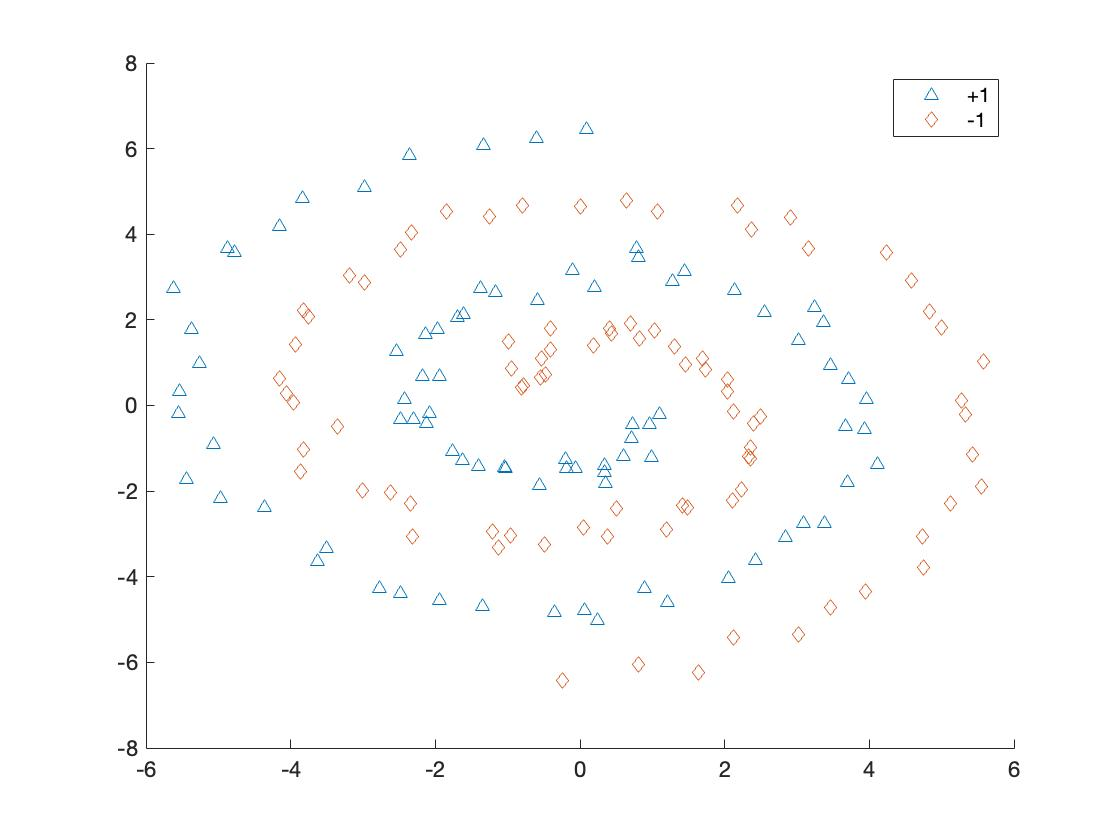
\includegraphics[width=0.9\linewidth]{training_data.jpg}\\
Fig1: Two spiral data sets (training)
\end{center}
As we mentioned in Section 2, our optimization problem is:
\begin{align}
\min_{\alpha_1,\cdots,\alpha_n}&\quad \frac{1}{2}\sum_{i,j}\alpha_i\alpha_jy_iy_jK_{ij}-\sum_{i=1}\alpha_i\\
s.t. &\quad \sum^n_{i=1}\alpha_iy_i=0\\
&\quad \forall i\ \alpha_i\ge0\\
&\quad \forall i\ C-\alpha_i\ge0
\end{align}
In this section, some numerical results will be reported to verify the efficiency of our algorithm. We follow the terminate idea suggested by Wang and Pu(2013)\upcite{Ref9} if:
\begin{align}
||\nabla f_k-\nabla c_\epsilon(x_k)^T\lambda_k-\nabla c_I(x_k)^T\mu_k||_2\le10^{-6}\\
||(c_\epsilon(x_k),max\{-c_I(x_k),0\})||_2\le10^{-6}
\end{align}
The parameters are chosen as: $\tau=0.5$, $\eta=0.1$, $\pi_0=1$, $\epsilon=10^{-4}$ and we initialize $\bm{\alpha}_0=(0,0,\cdots,0)^T$, $\lambda_0=0.5$ and $\bm{\mu}_0=(0.5,0.5,\cdots,0.5)^T$ where length of $\bm{\mu}$ is 2$\times$numbers of data. We then use Line Search SQP algorithm with flexible penalty functions mentioned in Section 3 to get optimized $\bm{\alpha}$s and classify 170 testing data:
\begin{center}
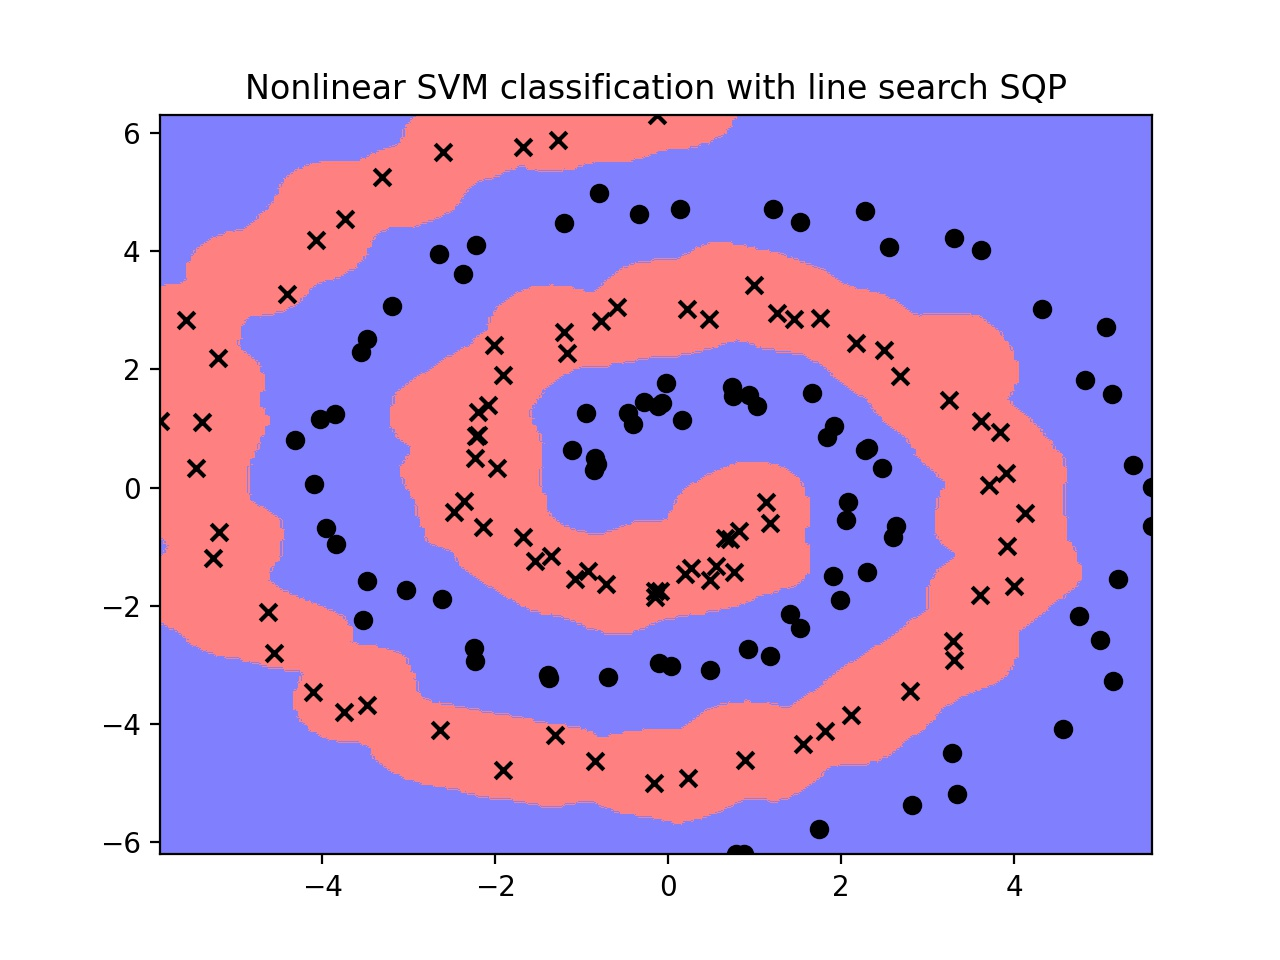
\includegraphics[width=0.9\linewidth]{testing_data_py.jpg}\\
Fig2: Two spiral data sets (testing)
\end{center}
As it is shown in Fig2, we classify the testing data with 0 testing error which shows succeed in optimizing $\alpha$ in our dual SVM problem.

\subsection{Convergence Result}
According to Huang and Madden(2015)\upcite{Ref4},  global convergence can be expected if following assumptions are satisfied:
\begin{enumerate}
\item $\{x_k\}$ and $\{x_k+\alpha p_k\}$ are contained in a compact and convex set $D$.
\item The objective function $g$ and the constraint functions $c_\epsilon$, $c_I$ are twice continuously differentiable on an open set containing $D$.
\item There exists an $M>0$ such that the Hessian matrices $H_k$ satisfy $||H_k||_2\le M$ for all k.
\end{enumerate}
The first condition means each subsequence of compact set is convergenct, that is, $\{x_k\}$ generated by algorithm should be converged. 
\begin{center}
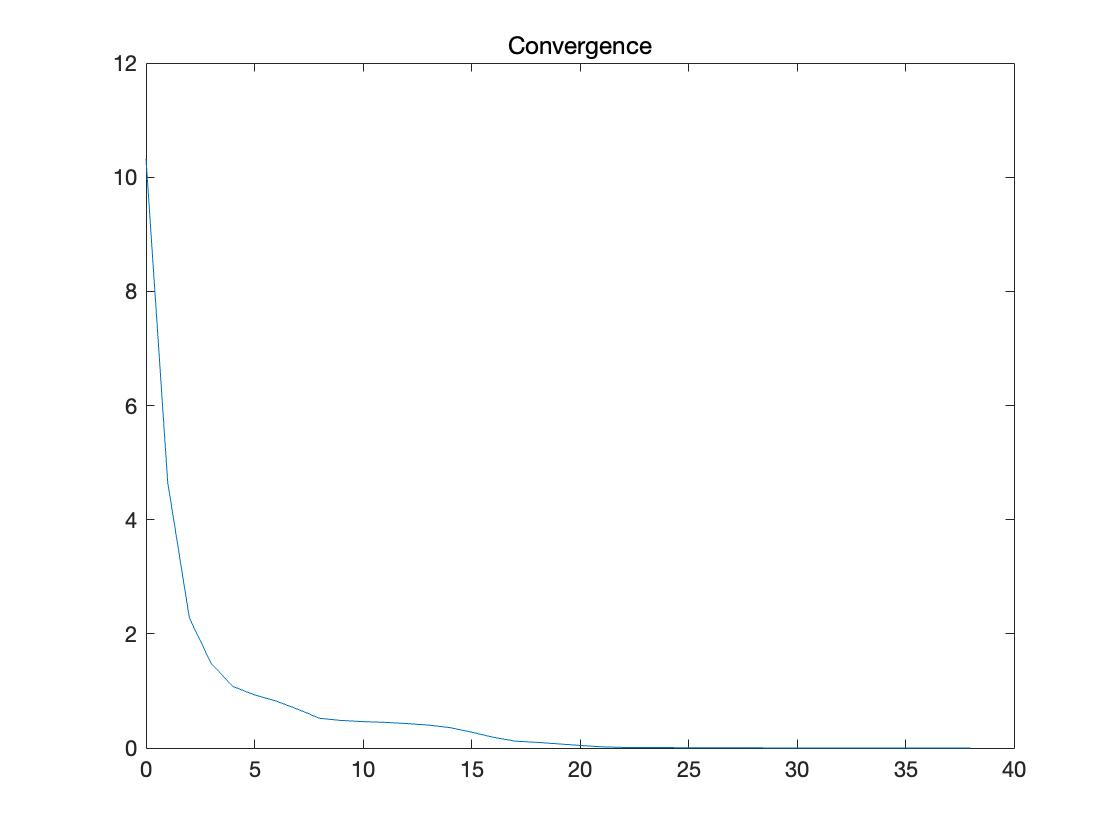
\includegraphics[width=0.9\linewidth]{convergence.jpg}\\
Fig3: Convergence of $\{x_k\}$
\end{center}
Fig3 proved that our algorithm generates converged $\{x_k\}$, which satisfy the first condition. As to the second condition, from function (58)-(61) we know that both $c_\epsilon$ and $c_I$ are twice continuously differentiable. Damped BFGS algorithm ensures each approximated hessian matrix is positive definite and finally close to the real hessian, which satisfy the third condition. To conclude, global convergence can be expected for our problem.\\

Besides, according to Boggs and Tolle(1995)\upcite{Ref1}, to ensure global convergence, a merit function $\phi$, which measures progress, whose reduction implies the reduction to an optimal point, must used throughout the iteration process in SQP algorithm. Here in our flexible line search SQP algorithm, we use $l_1$ penalty function as our merit function in each iteration to check whether the trial step should be accepted, thus global convergence could be ensured.\\

Boggs and Tolle\upcite{Ref1} combined line search SQP with BFGS method, where the choice of matrix $H_k$ is a finite difference approximation of the Hessian of the Lagrangian in each iteration, and named this algorithm as "PSB-SQP" algorithm. Another scheme, which they called the Powell-SQP method, is to use damped BFGS to ensure a positive definite approximated Hessian in each iteration. To make sure the convergence rate, Boggs and Tolle\upcite{Ref1} has given a theorem of local convergence properties.\\

To discuss convergence of line search SQP algorithm, the asymptotic rate of convergences play an important role. The convergence can be investigated with Q-convergence, the general Q-convergence is defined as:
\begin{align}
\frac{||x_{k+1}-x^*||}{||x_k-x^*||^p}\le M,\ M>0,\ \forall k\ sufficiently\ large,\ p>1
\end{align}
Q-linear convergence is defined:
\begin{align}
\frac{||x_{k+1}-x^*||}{||x_k-x^*||^p}< M,\ r\in(0,1),\ \forall k\ sufficiently\ large
\end{align}
We will also encounter a measure of the average rate of convergence called the $R-rate$. A sequence ${x_k}$ converges $R-linearly$ if the sequence $\{||x_k-x^*||\}$ is bounded by a Q-linearly convergence sequence.\\

There are two relationships between $Q-rate$ and $R-rate$. First, $m$-step $Q-linear$ convergence implies an $R-linear$ rate of convergence. Secondly, a sequence of $Q-rate$ vectors indicates the same $R-rate$ of convergence of its components(Boggs and Tolle, 1995).


~\\
\textbf{Theorem 4.1.1}  Suppose that $H_k$ is positive definite and let $H_0$ be an initial positive definite matrix. Suppose that the sequence $\{(x_k,\lambda_k)\}$ is generated by the SQP algorithm with sequence of matrix approximated by the BFGS update(57). Then, if $||x_0-x^*||$ and $||H_0-H^*||$ are sufficiently small and $\lambda_0$ is appropriate, the sequence $\{H_k\}$ is uniformly continuous and if
\begin{align}
\lim_{k\to\infty} \frac{||P^k(H_k-H*)(x_{k+1}-x_k)||}{||(x_{k+1}-x_k)||}=0
\end{align}
where
\begin{align}
P(x)=I-\nabla h(x)[\nabla h(x)^T\nabla h(x)]^{-1}\nabla h(x)^T
\end{align}
The iterates $(x_k,\lambda_k)$ converge superlinearly to the optimal solution. In addition the \textbf{x}-iterates converge superlinearly and the multipliers converge R-superlinearly.\\

Based on our numerical result generated by MATLAB, we plot Q-convergence of generated $\{x_k\}$. When p=1:
\begin{center}
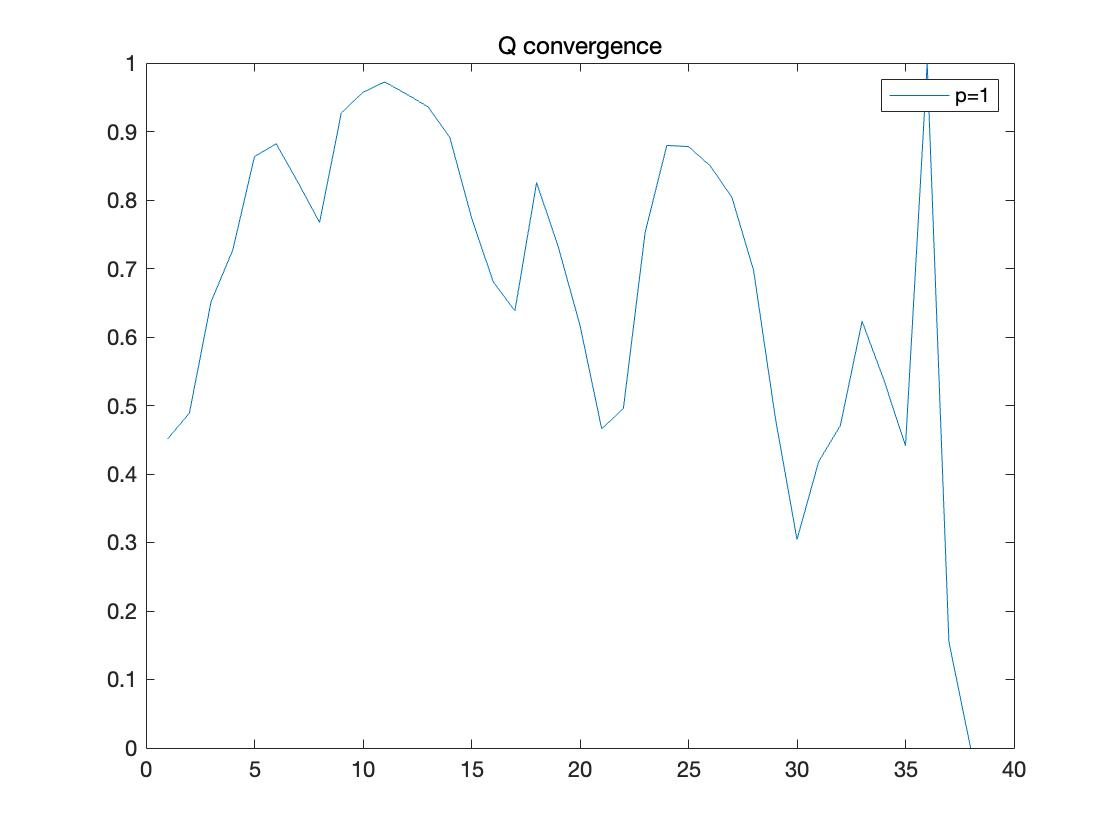
\includegraphics[width=0.9\linewidth]{p1.jpg}\\
Fig4: Q-linear convergence 
\end{center}
From Fig4 we can observe that all Q-convergence rate is from 0 to 1, which shows the algorithm converges at least a linear rate. When p=1.4 and p=2, we have:
\begin{center}
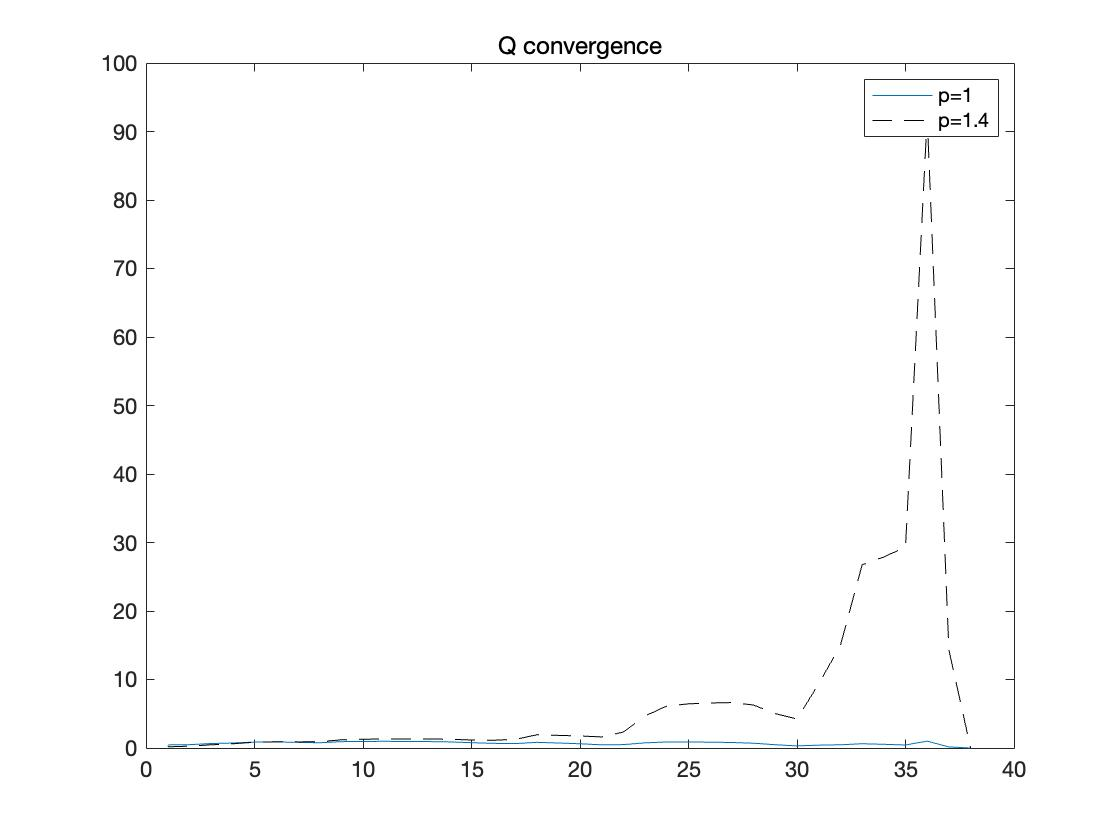
\includegraphics[width=0.9\linewidth]{p14.jpg}\\
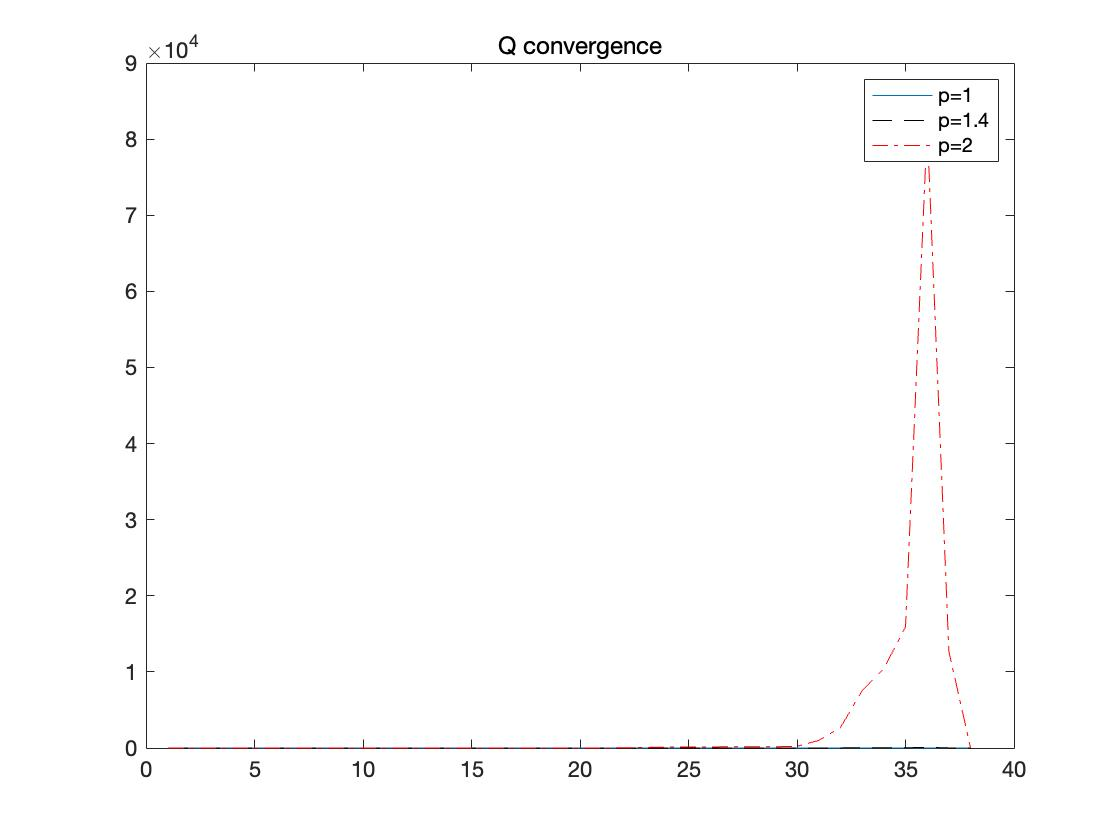
\includegraphics[width=0.9\linewidth]{p2.jpg}\\
Fig5: Q-convergence 
\end{center}
As we can see in Fig5, when p=1.4 and p=1.5, Q-convergence could not be bounded by a fixed M. To conclude, the algorithm converges linearly.\\

Combined with theorem mentioned before, we could observe that \textbf{x}-iterates has a local Q-superlinear convergence rate and the Lagrange multipliers has a local R-superlinear convergence rate. Through our numerical result and the assumption raised by Huang and Madden, $\{x_k\}$ converges globally and linearly.

\subsection{Performance complexity}
The CPU time of our algorithm costs 14.56 seconds and the memory used is 7591537.56 kb. In the algorithm we use two nested while loop, one is update variable until max iterations or satisfies stopping criteria, the other one is in each iteration, we backtracking to find an acceptable step length. Set we iterate n times and in each iteration, we backtracking m times, then the time complexity of our algorithm is O(nlog2m).

\section{Summary}
This report classifies random spiral data  with support vector machine, where a flexible line search SQP algorithm used to do the optimization.\\


The basic idea of SQP algorithm is to construct a quadratic programming subproblem in each iteration, and then to use the solution to this subproblem to construct a better approximation of $x_{k+1}$. SQP may share the characteristics of Newton-like methods, converge rapidly when the iterates are close to the solution. To decide whether the trial step is acceptable, a $l_1$ penalty function used as merit function in this report. Besides, this report use BFGS to approximate $H_k$ in each step, which is improved by Damped BFGS to ensure a positive definite Hessian. This algorithm named Powell-SQP by Boggs and Tolle in 1995.\\

This algorithm performs well since the trained classifier classified the testing data with 0 testing error.

\newpage
\section{Appendix}
Appendix shows the MATLAB code of implemented optimization method and classification problem.\\
~\\
\textbf{no\_project.m:}\\
We generate two different types of random spiral data as training data and testing data, use Line Search SQP algorithm to optimize the constraint optimization problem in SVM and use the trained alphas to classify testing data in this package.
\begin{lstlisting}
%%
clc; clear;
load seamount
C=10; % regularzation parameter

%% SVM
% generate data
[xTr, yTr, xTe, yTe]=sprialdata(170);

figure;
scatter(xTr(yTr==1,1),xTr(yTr==1,2),'^')
hold on
scatter(xTr(yTr~=1,1),xTr(yTr~=1,2),'d')
legend('+1','-1');

% compute gaussian kernel matrix: K
sigma=10;
K=gaussK(xTr,xTr,sigma);

yTr=yTr'; % now yTr:n*1
% dual optimization problem
A=(yTr*yTr').*K; % n*1 1*n .* n*n --> n*n

F.f=@(alpha) 0.5*alpha'*A*alpha-sum(alpha);
F.df=@(alpha) A*alpha-ones(size(yTr,1),1);
F.d2f=@(alpha) A;

c.h=@(alpha) alpha'*yTr;
c.dh=@(alpha) yTr';

alpha0=zeros(size(xTr,1),1);
lambda0=0.5;
mu0=0.5*ones(2.*size(xTr,1),1);

C_soft=C*ones(size(alpha0,1),size(alpha0,2)); % use soft margin

I.h=@(alpha) [alpha;C_soft-alpha]';
I.dh=@(alpha) [eye(size(alpha0,1)),-1*eye(size(alpha0,1))]';

% optimization alphas
[xMin,fMin,info,iter,mu_k]=sqpLine(F,c,I,alpha0,lambda0,mu0);


%%
[bias]=recoverBisas(K,yTr,xMin,C);
svmclassify=@(x) (xMin.*yTr)'*gaussK(xTr,x,sigma)+bias;

predsTr=svmclassify(xTr);
pred_err=length(yTr(yTr~=sign(predsTr')))/length(yTr)

predsTe=svmclassify(xTe);
pred_err_te=length(yTe(yTe~=sign(predsTe)))/length(yTe)

figure;
scatter(xTe(sign(predsTe)==1,1),xTe(sign(predsTe)==1,2))
hold on
scatter(xTe(sign(predsTe)~=1,1),xTe(sign(predsTe)~=1,2))
legend('+1','-1');

% visclassifier(svmclassify,xTe,yTe)

%% convergence

con_SQP=convergenceHistory(info,[],F,2);
figure;
plot(0:length(con_SQP.x)-1,con_SQP.x);hold on;title('Convergence');

p=1;
rs1=(con_SQP.x(2:end))./((con_SQP.x(1:end-1)).^p);
ps=1.4;
rss=(con_SQP.x(2:end))./((con_SQP.x(1:end-1)).^ps);
p=2;
rs2 = (con_SQP.x(2:end))./((con_SQP.x(1:end-1)).^p); 
figure, plot(rs1); hold on; title('Q convergence'); legend('p=1')
figure, plot(rs1); hold on; plot(rss,'k--'); title('Q convergence'); legend('p=1',['p=' num2str(ps)])
figure, plot(rs1); hold on; plot(rss,'k--'); plot(rs2,'r-.'); title('Q convergence'); legend('p=1',['p=' num2str(ps)],'p=2')




\end{lstlisting}
~\\
\textbf{spiraldata.m:}\\
In this package we generate random spiral data.

\begin{lstlisting}
function [xTr, yTr, xTe, yTe]=sprialdata(N)
rng(24) %24
r=linspace(1,2*pi,N);
xTr1=[sin(2.*r).*r;cos(2.*r).*r]';
xTr2=[sin(2.*r+pi).*r;cos(2.*r+pi).*r]';
xTr=[xTr1;xTr2];
xTr=xTr+normrnd(0,1,size(xTr,1),size(xTr,2))*0.2;
yTr=[ones(1,N),-1.*ones(1,N)];

xTe=xTr(1:2:end,:);
yTe=yTr(:,1:2:end);
xTr=xTr(2:2:end,:);
yTr=yTr(:,2:2:end);
\end{lstlisting}

~\\
\textbf{sqpLine.m:}\\
In this package, we use Line Search SQP with a flexible penalty function to solve the optimization problem in SVM.
\begin{lstlisting}
function [xMin,fMin,info,iter,mu_k]=sqpLine(F,c,I,x0,lambda0,mu0)
% F: objective function
% c: equality constraints
% i: inequality constraints
% x0: initial points
% lambda0: initial lambda
% k: iteration numbers
maxIter=500;
tau=0.5;
eta=0.1;
sigma=1;
pi_k=1/sigma;
x_k=x0;
% equality
lambda_k=lambda0; 
l=length(lambda0);
% inequality
mu_k=mu0;
m=length(mu0);
epsilon1=1e-6; epsilon2=1e-6;
% objective
f_k=F.f(x_k);
df_k=F.df(x_k);
% equality
h_k=c.h(x_k);
Ae_k=c.dh(x_k);
% inequality
v_k=I.h(x_k);
Ai_k=I.dh(x_k);
A_k=[Ae_k;Ai_k];
% initial H0 for BFGS
H_k=eye(length(x0));
% initial information
info.xs=x0;
info.lambdas=lambda0;

iter=0;
while(iter<maxIter)
    % slove subsequence quadratic programme
    [pk,lambda,mu]=qpsubp(df_k,H_k,Ae_k,h_k,Ai_k,v_k);
    lambda_k=lambda;
    mu_k=mu;
    mp1=norm(h_k,2)+norm(max(-v_k,0),2);
    dL=dLagrange(lambda_k,mu_k,df_k,Ae_k,Ai_k);

    if (norm(dL,2)<epsilon1)&&(mp1<epsilon2)
        break;
    end
    
    % penalty parameter update, set mu=1/sigma
    mu_eps=1e-4;
    r_k=max(norm(lambda_k,inf),norm(mu_k,inf));

    if (pi_k>r_k)
        pi_k=pi_k;
    else
        pi_k=r_k+mu_eps;
    end

    % backtracking line search with algorithm 18.3 method
    Phi.phi=@(x,pi_k) F.f(x)+pi_k*(norm(c.h(x),1)+norm(max(-I.h(x),0),1));
    Phi.dphi=@(x,pi_k,pk) F.df(x)'*pk+pi_k*(norm(c.h(x),1)+norm(max(-I.h(x),0),1));
    i=0;
    while(i<=20)
        if(Phi.phi(x_k+tau^i*pk,pi_k)-Phi.phi(x_k,pi_k)<eta*tau^i*Phi.dphi(x_k,pi_k,pk))
            mk=i;
            break;
        end
        i=i+1;
        if (i==20)
            mk=10;
        end
    end
    alpha_k=tau^mk;
    x_k_1=x_k+alpha_k*pk;
    df_k_1=F.df(x_k_1); % new gradient objective function-not update yet
    Ae_k_1=c.dh(x_k_1); % new gradient equality constrains-not update yet
    Ai_k_1=I.dh(x_k_1); % new gradient inequality constrains-not update yet

    h_k=c.h(x_k_1); % update equality constrains
    v_k=I.h(x_k_1); % update inequality constrains
    A_k=[Ae_k_1;Ai_k_1]; % combine equality with inequality

    p_lambda=pinv(A_k)'*df_k_1;

    lambda_k=p_lambda(1:l);
    mu_k=p_lambda(l+1:l+m);

    % damped BFGS updating
    s_k=x_k_1-x_k;
    y_k=dLagrange(lambda_k,mu_k,df_k_1,Ae_k_1,Ai_k_1)-dLagrange(lambda_k,mu_k,df_k,Ae_k,Ai_k);

    if(s_k'*y_k>0.2*s_k'*H_k*s_k)
        theta=1;
    else
        theta=0.8*s_k'*H_k*s_k/(s_k'*H_k*s_k-s_k'*y_k);
    end
    rk=theta*y_k+(1-theta)*H_k*s_k;
    H_k=H_k+rk*rk'/(s_k'*rk)-(H_k*s_k)*(H_k*s_k)'/(s_k'*H_k*s_k);

    % update
    x_k=x_k_1;
    df_k=df_k_1;
    Ae_k=Ae_k_1;
    Ai_k=Ai_k_1;
    info.xs=[info.xs,x_k];
    info.lambdas=[info.lambdas,lambda_k];
    iter=iter+1;

end
xMin=x_k;
fMin=F.f(x_k);

%==================== gradient Lagrange nabla L(x,lambda,mu) ===============
function dL=dLagrange(lambda,mu,df,Ae,Ai)
m1=size(Ai,1); l1=size(Ae,1);
if(l1==0)
    dL=df-Ai'*mu;
end
if(m1==0)
   dL=df-Ae'*lambda; 
end
if(l1>0&&m1>0)
    dL=df-Ae'*lambda-Ai'*mu;
end
\end{lstlisting}

~\\
\textbf{recoverbias.m:}\\
In this package, we calculate bias term of hyperplane after optimized alphas obtained.
\begin{lstlisting}
function [bias]=recoverBisas(K,yTr,alpha,C)
%  function bias=recoverBias(K,yTr,alpha,C);
%  Solves for the hyperplane bias term, which is uniquely specified by the 
%  support vectors with alpha values 0<alpha<C
%  This is most stable if we pick an alpha_i that is furthest from C and 0
%     
%  INPUT:
%  K : nxn kernel matrix
%  yTr : nx1 input labels
%  alpha  : nx1 vector of alpha values
%  C : regularization constant
%     
%  Output:
%  bias : the scalar hyperplane bias of the kernel SVM specified by alphas
gap=abs(alpha-0.5*C);
alpha_index=find(gap==min(gap));
bias=yTr(alpha_index)-(yTr'.*alpha')*K(:,alpha_index);
\end{lstlisting}




















\newpage
\begin{thebibliography}{99}
\bibitem{Ref1}
Boggs, P. T., \& Tolle, J. W. (1995). Sequential quadratic programming. Acta numerica, 4, 1-51.
\bibitem{Ref2}
Cristianini, N. \& Shawe-Taylor, J. (2000). An Introduction to Support Vector Machines. Cambridge University Press
\bibitem{Ref3}
Howley, T., Madden, M.G. The Genetic Kernel Support Vector Machine: Description and Evaluation. Artif Intell Rev 24, 379–395 (2005). https://doi.org/10.1007/s10462-005-9009-3
\bibitem{Ref4}
Huang, M., \& Pu, D. (2015). A line search SQP method without a penalty or a filter. Computational and Applied Mathematics, 34(2), 741-753.
\bibitem{Ref5}
Trevor, H., Robert, T., \& Jerome, F. (2009). The elements of statistical learning: data mining, inference, and prediction.
\bibitem{Ref6}
Smola, A. J., Schölkopf, B., \& Müller, K. R. (1998). The connection between regularization operators and support vector kernels. Neural networks, 11(4), 637-649.
\bibitem{Ref7}
Wright, S., \& Nocedal, J. (1999). Numerical optimization. Springer Science, 35(67-68), 7.
\bibitem{Ref8}
Zhu, X., \& Pu, D. (2012). Sequential quadratic programming with a flexible step acceptance strategy. Applied Mathematical Modelling, 36(9), 3992-4002.
\bibitem{Ref9}
Wang, B., \& Pu, D. (2013, September). Flexible penalty functions for SQP algorithm with additional equality constrained phase. In Proceedings of the 2013 International Conference on Advanced Mechatronic Systems (pp. 22-27). IEEE.


\end{thebibliography}

\end{spacing}
\end{document}